% E3 paper figure -- one double-column figure (PDF: 515.5 x 374.4 pt = 7.16 x 5.20 in;
% \textwidth, inserted at 100 % scale). Fonts: STIX (Times-compatible), embedded TrueType.
% Copy results/E3/figures/paper/paper_fig_e3_dynamic_coordination_combined.pdf
% (also in benchmark/paper_assets/E3/) to the manuscript's figures/ folder.
% Supersedes the four single-column figures (fig:e3_concurrent_tracking,
% fig:e3_ee_to_base_frequency, fig:e3_ee_to_base_response, fig:e3_base_to_ee_response).
% Not compiled against the manuscript (manuscript not available to the generator).

\begin{figure*}[t]
    \centering
    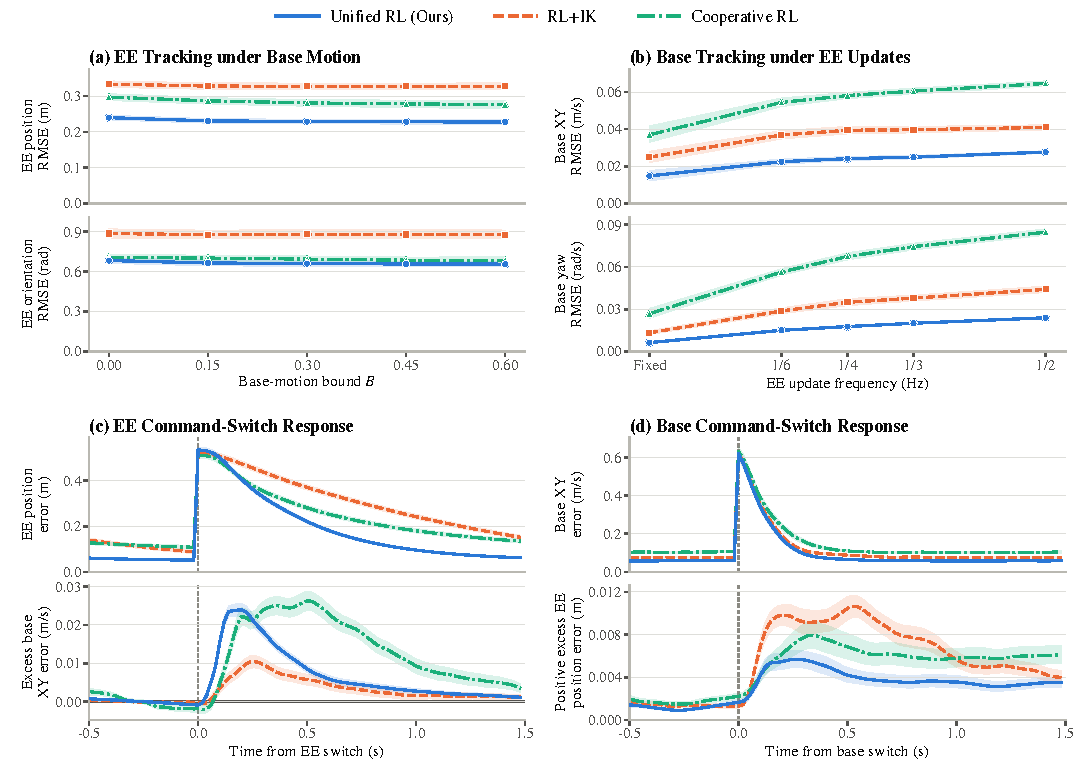
\includegraphics[width=\textwidth]
        {figures/paper_fig_e3_dynamic_coordination_combined.pdf}
    \caption{Dynamic whole-body coordination on the random discrete full-pose
    benchmark. EE targets are full 6-DoF poses drawn from the training pose set
    and held between updates; base commands are piecewise constant within the
    symmetric bound $B$ on planar velocity (m/s) and yaw rate (rad/s).
    (a)~EE position and orientation RMSE versus $B$, with EE targets updated
    every 2\,s. (b)~Base XY velocity and yaw-rate RMSE versus EE update
    frequency, with a stationary base command ($B=0$; ``Fixed'' holds one
    target). (a)--(b) are 3--30\,s RMSEs under concurrent command streams.
    (c)--(d) are responses aligned to isolated command switches (no other
    command change within $[-1.0,1.5)$\,s), using only switches present for all
    three controllers. (c)~EE-target switches ($B=0$, 2\,s updates; 1{,}200
    switches): absolute EE position error and signed excess base XY velocity
    error. (d)~Base-velocity switches with the EE target fixed ($B=0.60$; 652
    switches in 90 trials): absolute base XY velocity error and mean positive
    excess EE position error, $\max(e_i(t)-\bar{e}_{i,\mathrm{pre}},0)$
    averaged over switches, which is nonzero before $t=0$ because fluctuations
    are rectified. Excess errors are relative to each switch's mean over
    $[-0.5,0)$\,s and measure induced change, not absolute accuracy. The
    positive-excess presentation in (d) and the shared-switch restriction were
    chosen after data collection. Lines are means over 100 paired simulation
    trials, with switches averaged within each trial; bands are 95\%
    paired-bootstrap confidence intervals.}
    \label{fig:e3_dynamic_coordination}
\end{figure*}
